\documentclass[12pt]{article}

%%% Packages
\usepackage[margin=2.5cm]{geometry}
\usepackage{setspace}
\usepackage{lineno}
\usepackage{booktabs}
\usepackage{longtable}
\usepackage{graphicx}
\usepackage{amsmath}
\usepackage{textcomp}
\usepackage[hidelinks]{hyperref}

%%% Graphics path
\graphicspath{{figures/}}

%%% Double spacing and line numbers
\doublespacing
\linenumbers

%%% Begin document
\begin{document}

%% ============================================================
%% TITLE PAGE
%% ============================================================

\begin{titlepage}
\centering
\vspace*{2cm}

{\LARGE\bfseries Global, Regional, and National Quality of Care Index for Drug-Susceptible Tuberculosis, 1990--2021: A Systematic Analysis of the Global Burden of Disease Study\par}

\vspace{2cm}

{\large\textbf{Authors:} [Author list to be finalised]\par}

\vspace{1cm}

{\large\textbf{Correspondence:} [Corresponding author details]\par}

\vspace{1cm}

{\large\textbf{Word count:} \textasciitilde 4800\par}

\vspace{1cm}

{\large\textbf{Keywords:} tuberculosis, quality of care, Global Burden of Disease, composite index, health system performance, drug-susceptible tuberculosis\par}

\vfill

\end{titlepage}

%% ============================================================
%% ABSTRACT
%% ============================================================

\section*{Abstract}

\textbf{Background:} Tuberculosis (TB) remains a leading cause of infectious disease mortality worldwide, yet no composite, population-level metric exists to assess the quality of care for drug-susceptible TB (DS-TB) across countries and over time. Existing indicators capture single dimensions of the care cascade, limiting their utility for cross-national benchmarking and temporal monitoring. We aimed to develop and validate a Quality of Care Index (QCI) for DS-TB using data from the Global Burden of Disease (GBD) Study 2021.

\textbf{Methods:} We used GBD 2021 estimates of incidence, prevalence, mortality, disability-adjusted life-years (DALYs), years of life lost (YLLs), and years lived with disability (YLDs) for DS-TB across 204 countries and territories, 31 years (1990--2021), five age groups, and both sexes. Three component ratios were constructed: the mortality-to-incidence ratio (MIR), the YLL-to-YLD ratio (YLLtoYLD), and the DALY-to-prevalence ratio (DALtoPER). Principal component analysis (PCA) was applied to the standardised ratios; the first principal component (PC1), explaining 87.98\% of variance, was inverted and rescaled to 0--100 so that higher scores denote better care quality. Uncertainty was propagated via 1000-draw Monte Carlo simulation using GBD uncertainty intervals. Temporal trends were quantified with average annual percent change (AAPC) from log-linear regression. Construct validity was assessed through Spearman correlation with the Socio-demographic Index (SDI).

\textbf{Findings:} Global age-standardised QCI rose from 91.87 (95\% uncertainty interval [UI] 90.57--93.03) in 1990 to 95.46 (94.68--96.13) in 2021, corresponding to an AAPC of +0.119\% (95\% CI +0.116 to +0.123). Of 195 countries with complete data, 189 improved and six declined between 1990 and 2021. In 2021, QCI ranged from 82.39 (Afghanistan) to 99.94 (Bermuda); 130 countries exceeded a QCI of 95. North America recorded the highest regional QCI (97.82), while Sub-Saharan Africa recorded the lowest (93.11). A clear SDI gradient was observed (Spearman rho = 0.768, p = 2.03 $\times$ 10\textsuperscript{--31}), with low-SDI settings converging faster (AAPC +0.135\%) than high-SDI settings (+0.093\%). Females had higher QCI than males globally (96.13 vs 94.88), and children aged 5--14 years had the highest age-specific QCI (97.82) while those under 5 years had the lowest (92.61). Six countries experienced net QCI declines, led by Zimbabwe (--7.82 points) and Lesotho (--6.61 points).

\textbf{Interpretation:} Substantial but uneven progress in DS-TB care quality has occurred over three decades. Persistent gaps in Sub-Saharan Africa, low-SDI countries, males, and children under 5 years highlight populations requiring targeted investment. The QCI offers a reproducible, composite benchmark for monitoring TB care quality at the population level and can inform resource allocation toward the 2030 End TB Strategy targets.

\textbf{Funding:} None.

\newpage

%% ============================================================
%% INTRODUCTION
%% ============================================================

\section{Introduction}

Tuberculosis (TB) remains among the foremost global health challenges of the twenty-first century. The World Health Organization (WHO) estimated 10.6 million new cases and 1.3 million deaths attributable to TB in 2022, making it the leading single-agent infectious cause of mortality worldwide.\textsuperscript{1} Despite the availability of effective first-line treatment regimens for drug-susceptible TB (DS-TB), outcomes vary enormously between and within countries, reflecting profound disparities in health system capacity, diagnostic access, treatment adherence support, and broader socioeconomic determinants of health.\textsuperscript{2,3}

Monitoring the quality of TB care at the population level is essential for tracking progress toward the End TB Strategy targets, which call for a 90\% reduction in TB deaths and an 80\% reduction in incidence by 2030 relative to 2015 levels.\textsuperscript{4} However, existing metrics for TB programme performance tend to capture single dimensions of the care cascade. The case detection rate quantifies the proportion of estimated incident cases that are notified, while the treatment success rate measures the fraction of notified patients who complete therapy. Neither metric, on its own, reflects the full spectrum of care quality -- from timely diagnosis through effective treatment to avoidance of premature mortality and residual morbidity.\textsuperscript{5}

The Healthcare Access and Quality (HAQ) Index, developed as part of the Global Burden of Disease (GBD) Study, offers an important precedent for composite health system performance measurement.\textsuperscript{6} By synthesising mortality-to-incidence ratios across amenable causes of death, the HAQ Index has enabled cross-national and temporal comparisons of personal healthcare access and quality. Nevertheless, the HAQ Index does not incorporate disease-specific morbidity dimensions and treats each amenable cause equally rather than capturing the distinct care cascade relevant to specific conditions such as TB.

A composite Quality of Care Index (QCI) that integrates mortality, morbidity, and disability dimensions specific to DS-TB would fill a critical gap in the global TB monitoring landscape. Such a metric could enable identification of countries and populations where care quality lags, inform priority-setting for health system strengthening, and provide a single summary measure for benchmarking progress. Importantly, because the QCI is constructed from population-level outcome ratios, it functions as an outcome-based proxy for the net effectiveness of DS-TB care systems rather than a direct measure of clinical care processes;\textsuperscript{28} it captures the combined influence of healthcare delivery, diagnostic access, treatment infrastructure, and broader socioeconomic determinants on TB outcomes.

In this study, we developed and applied a composite QCI for DS-TB using GBD 2021 estimates for 204 countries and territories over the period 1990--2021. We constructed the index from three outcome-based ratios reflecting case fatality (mortality-to-incidence ratio), the burden of premature death relative to disability (YLL-to-YLD ratio), and the overall disease burden per prevalent case (DALY-to-prevalence ratio). We describe global, regional, and national trends; examine patterns by age and sex; assess convergence across development levels; and validate the index against the Socio-demographic Index.

%% ============================================================
%% METHODS
%% ============================================================

\section{Methods}

\subsection{Data source and scope}

We used publicly available estimates from the GBD 2021 Study for DS-TB, encompassing six epidemiological indicators: incidence, prevalence, mortality, DALYs, YLLs, and YLDs. Estimates were available for 204 countries and territories, 31 calendar years (1990--2021), five age groups (under 5, 5--14, 15--49, 50--69, and 70+ years) plus age-standardised and all-ages aggregates, and three sex categories (male, female, and both sexes). The GBD methodology for estimating DS-TB burden has been described in detail elsewhere.\textsuperscript{7,8,9} Briefly, the GBD uses a Bayesian meta-regression framework (DisMod-MR 2.1) that synthesises data from vital registration systems, verbal autopsy studies, disease notification records, population-based surveys, and published literature to produce internally consistent estimates with 95\% uncertainty intervals (UIs).

\subsection{Component ratios}

We constructed four candidate ratios to capture different dimensions of DS-TB care quality. The \textbf{mortality-to-incidence ratio (MIR)} was defined as the age-standardised DS-TB mortality rate divided by the age-standardised incidence rate, reflecting case fatality and thus the effectiveness of diagnosis and treatment. The \textbf{YLL-to-YLD ratio (YLLtoYLD)} was defined as the YLL rate divided by the YLD rate, capturing the relative contribution of premature mortality versus disability in the overall disease burden; a lower value indicates that a greater proportion of the burden stems from morbidity rather than early death. The \textbf{DALY-to-prevalence ratio (DALtoPER)} was calculated as the DALY rate divided by the prevalence rate, representing the average disease burden per prevalent case; lower values indicate less severe outcomes per case. A fourth ratio, the \textbf{prevalence-to-incidence ratio (PERtoINC)}, was initially considered as an indicator of disease duration, but was subsequently excluded on the basis of sensitivity analysis.

\subsection{Principal component analysis}

We applied principal component analysis (PCA) to derive a single composite score from the component ratios. All ratios were first standardised using z-score transformation (zero mean, unit variance). PCA was trained on age-standardised, both-sexes data across all countries and years. In the three-component model (MIR, YLLtoYLD, DALtoPER), the first principal component (PC1) explained 87.98\% of total variance. PCA loadings on PC1 were: MIR 28.07\%, YLLtoYLD 36.08\%, and DALtoPER 35.85\%, indicating that all three ratios contributed substantially and approximately equally, with the two burden-oriented ratios carrying slightly greater weight.

Because PCA is agnostic to the direction of ``better'' quality, PC1 was inspected for its correlation with MIR (Pearson r = 0.861 before sign correction). Since higher values of all three ratios denote worse outcomes, PC1 was inverted (multiplied by --1) so that higher scores correspond to better care quality. The inverted PC1 scores were then rescaled to a 0--100 range using global minimum-maximum normalisation across all country-year observations to produce the final QCI.

The transformation parameters (means, standard deviations, PCA loadings, and min-max bounds) derived from the training set (age-standardised, both-sexes stratum) were applied uniformly to all demographic strata (specific age groups and sex categories) to ensure cross-stratum comparability.

\subsection{Index scope and component collinearity}

The three component ratios share GBD outcome quantities by construction: deaths appear in the numerators of both MIR and the YLL component, while prevalence appears in the denominator of DALtoPER and contributes to the YLD calculation. The component ratios are therefore mathematically related rather than measurement-independent. The high proportion of variance captured by PC1 (87.98\%) is consistent with this structural relationship and indicates that a single common factor --- interpretable as the intensity of fatal versus non-fatal DS-TB burden --- dominates the joint variation of the three ratios. Accordingly, the QCI is best understood as a smoothed composite of mortality-intensity rather than as a multidimensional measure of orthogonal care-quality domains. We retain the composite formulation because (i) PCA averages stochastic noise across three correlated GBD-modelled indicators rather than relying on any single ratio, (ii) the bounded 0--100 scale supports cross-location comparison and policy communication, and (iii) the sensitivity analyses reported below and elsewhere produce near-identical rankings under alternative parameterisations.

We also note explicitly that the term ``Quality of Care Index'' refers, throughout this study, to outcome-based, population-level performance and not to process-of-care indicators such as diagnostic timeliness, drug supply continuity, treatment adherence support, or service coverage. Such processes are reflected in the QCI only to the extent that they shape the modelled outcome ratios. We therefore frame the QCI as an outcome-based proxy for the net effectiveness of DS-TB care systems rather than as a direct measure of clinical care quality.

\subsection{Sensitivity analysis for component selection}

To assess the contribution of PERtoINC, we compared four-component and three-component PCA models. In the four-component model, PERtoINC contributed only 0.37\% to PC1 variance, and the variance explained by PC1 dropped from 87.98\% to 66.13\%. Country-level QCI scores from the two models were nearly identical (Spearman rho = 0.998, p $<$ 0.001), with 19 of 20 top-ranked and 20 of 20 bottom-ranked countries overlapping. On the basis of parsimony and negligible impact on rankings, the three-component model was selected as the primary specification.

\subsection{Uncertainty quantification}

Uncertainty in the QCI was propagated using Monte Carlo simulation with 1000 random draws. For each country-year observation, each of the six GBD input measures (Deaths, Incidence, YLLs, YLDs, DALYs, Prevalence) was sampled from a log-normal distribution parameterised so that the GBD point estimate was the median and the GBD 95\% UI bounds approximately bracketed the central 95\% of draws on the natural scale (i.e., $\log\mathrm{SD} = [\log(\text{upper}) - \log(\text{lower})] / [2 \times 1.96]$). Log-normal sampling was used in place of a symmetric-normal approximation because (i) GBD inputs are non-negative rates, so a normal distribution can produce negative draws that require ad hoc clipping, (ii) GBD UIs are typically asymmetric about the point estimate, and (iii) ratios of log-normal variables (e.g., MIR = Deaths / Incidence) are also log-normal, which is closer to GBD's underlying modelling framework than a ratio of normals. For each draw, the three component ratios were recalculated and the PCA transformation was applied using the fixed training parameters; the 2.5th and 97.5th percentiles of the resulting 1000 QCI values defined the 95\% UI for the QCI. The six measures were sampled independently within each country-year, which underestimates true uncertainty because GBD's modelling framework induces correlation between them; this is acknowledged as a limitation.

\subsection{Trend analysis}

Temporal trends were quantified using average annual percent change (AAPC), estimated from log-linear regression of QCI on calendar year: $\ln(\text{QCI}) = \beta_0 + \beta_1 \times \text{year}$. The AAPC was calculated as $(\exp(\beta_1) - 1) \times 100$, with 95\% confidence intervals derived from the $t$-distribution of $\beta_1$. Full-period (1990--2021) and recent-period (2010--2021) AAPCs were calculated for all locations.

\subsection{Validation}

Construct validity was assessed by Spearman rank correlation between country-level QCI in 2021 and the GBD Socio-demographic Index (SDI), a composite measure of per-capita income, educational attainment, and fertility rate.\textsuperscript{8,32} The SDI was selected as the primary external validator because it captures the socioeconomic determinants that underpin health system capacity.

\subsection{Ethical approval}

Ethical approval was not required for this study as it exclusively used publicly available, de-identified, aggregate data from the GBD 2021 Study.

\subsection{Role of the funding source}

This study received no external funding. The authors had full access to all data and had final responsibility for the decision to submit for publication.

%% ============================================================
%% RESULTS
%% ============================================================

\section{Results}

\subsection{Global trends}

Of the 204 countries and territories in the GBD 2021 dataset, 195 had complete data for all six epidemiological indicators across the full study period (1990--2021) and were included in the temporal trend analyses. The remaining nine locations lacked one or more indicators for specific years, precluding AAPC calculation, but were included in cross-sectional 2021 analyses where data were available.

Global age-standardised QCI for DS-TB increased from 91.87 (95\% UI 90.57--93.03) in 1990 to 95.46 (94.68--96.13) in 2021, representing an absolute gain of 3.59 points over 31 years (Table~1; Figure~1; Figure~3). The AAPC over the full period was +0.119\% (95\% CI +0.116 to +0.123), with a similar recent-period AAPC of +0.122\% (+0.114 to +0.129), indicating sustained improvement without acceleration or deceleration at the global level. The uncertainty width narrowed from 2.45 points in 1990 to 1.45 points in 2021, reflecting improved data availability and more precise GBD estimates over time.

All three component ratios declined between 1990 and 2021 at the global level. The MIR fell from 0.2304 to 0.1293, a 43.9\% reduction, indicating that a substantially smaller fraction of incident DS-TB cases resulted in death by 2021. The YLLtoYLD ratio fell from 16.49 to 9.19, a 44.3\% reduction, reflecting a shift in the composition of DS-TB burden from premature mortality toward non-fatal morbidity. The DALtoPER ratio decreased from 5.27 to 3.09, a 41.4\% reduction, indicating lower average disease burden per prevalent case. The broadly parallel declines across all three components suggest that improvement in DS-TB care quality has been multidimensional rather than driven by a single factor.

\subsection{Regional patterns}

All seven World Bank regions experienced QCI improvement between 1990 and 2021, although the magnitude and pace of gains varied substantially (Table~1; Figure~1). In 2021, North America had the highest regional QCI at 97.82 (95\% UI 97.44--98.15), followed by Europe and Central Asia at 97.38 (96.70--97.92) and East Asia and the Pacific at 96.92 (96.44--97.38). Sub-Saharan Africa had the lowest regional QCI at 93.11 (91.97--94.20), followed by South Asia at 94.98 (93.83--95.87). The gap between the highest and lowest regions was 4.70 points in 2021.

Latin America and the Caribbean recorded the largest absolute QCI gain (+4.62 points, from 91.20 to 95.82), with a full-period AAPC of +0.152\% (+0.131 to +0.174), the fastest of any region. South Asia also showed substantial improvement (+4.05 points), with the largest contributions from India and neighbouring countries. East Asia and the Pacific improved by 3.90 points, reflecting notable gains in China (QCI 94.21 to 98.68, +4.47 points). Sub-Saharan Africa, despite having the lowest absolute QCI, improved by 2.41 points with an AAPC of +0.103\% (+0.096 to +0.110).

North America showed a noteworthy pattern: while the full-period AAPC was +0.094\% (+0.073 to +0.116), the recent-period AAPC turned negative at --0.017\% (--0.028 to --0.005), indicating a recent deceleration or reversal in QCI gains. This pattern was driven primarily by the United States (recent AAPC --0.020\%, --0.033 to --0.008). Europe and Central Asia, by contrast, showed acceleration (recent AAPC +0.118\% vs full-period +0.084\%).

\subsection{Socio-demographic Index gradient}

A clear SDI gradient in QCI was observed in 2021 (Figure~2; Figure~3). High-middle SDI countries had the highest aggregate QCI at 98.12 (97.73--98.43), marginally exceeding the high-SDI group at 97.80 (97.38--98.15). Middle SDI countries scored 96.90 (96.35--97.38), low-middle SDI countries 94.45 (93.44--95.35), and low SDI countries 93.23 (92.04--94.18). The gap between the high and low SDI quintiles was 4.57 points.

The observation that high-middle SDI slightly surpassed high SDI may reflect the epidemiological composition of these groupings: high-middle SDI includes countries such as China (QCI 98.68) and Cuba (99.04) that have achieved exceptionally strong TB outcomes relative to their development level,\textsuperscript{29} while several high-SDI countries carry legacy burdens among ageing or marginalised populations.\textsuperscript{31}

Country-level validation confirmed a strong monotonic association between QCI and SDI (Spearman rho = 0.768, p = 2.03 $\times$ 10\textsuperscript{--31}; Pearson r = 0.712, p = 2.71 $\times$ 10\textsuperscript{--25}; n = 155 countries). Importantly, low-SDI countries exhibited faster QCI convergence (AAPC +0.135\%, +0.130 to +0.141) than high-SDI countries (+0.093\%, +0.083 to +0.103), suggesting a narrowing of the development-quality gap over time. All 45 high-SDI countries (100\%) achieved QCI above 90 in 2021, compared with 33 of 40 low-SDI countries (82.5\%).

\subsection{Country-level variation}

Country-level QCI in 2021 spanned a 17.55-point range, from 82.39 in Afghanistan (95\% UI 74.94--87.14) to 99.94 in Bermuda (Table~2). The top five countries were Bermuda (99.94), New Zealand (99.63), Malta (99.54), Antigua and Barbuda (99.31), and Luxembourg (99.16). The bottom five were Afghanistan (82.39), Lesotho (84.60), Zimbabwe (85.51), Marshall Islands (87.16), and the Central African Republic (87.17). The country-level mean QCI was 95.68 (SD 2.83), with a median of 96.38 and an interquartile range of 3.47 points.

Of 195 countries, 130 (66.7\%) achieved a QCI above 95, and only two (1.0\%) -- Afghanistan and Lesotho -- fell below 85. A total of 189 countries (96.9\%) experienced net QCI improvement between 1990 and 2021, with a mean change of +2.63 points and a maximum improvement of +12.66 points (Guatemala, from 81.21 to 93.87). Six countries experienced net QCI declines: Zimbabwe (--7.82, from 93.33 to 85.51; AAPC --0.357\%), Lesotho (--6.61, from 91.21 to 84.60; AAPC --0.263\%), Eswatini (--3.00, from 94.30 to 91.30; AAPC --0.069\%), Kenya (--0.99, from 89.59 to 88.60; AAPC --0.075\%), Libya (--0.55, AAPC --0.011\%), and Burkina Faso (--0.10, AAPC --0.009\%) (Figure~8).

Among the fastest-improving countries over the full period were Guatemala (AAPC +0.470\%), Rwanda (+0.432\%), Zambia (+0.353\%), Ethiopia (+0.342\%), and Afghanistan (+0.331\%). Several of these countries began from very low baselines, and the absolute magnitude of their improvements reflects concerted health system investment and programme scale-up.

\subsection{Age and sex patterns}

At the global level, females had higher QCI than males across all age groups in 2021 (Table~3; Figure~7). The global age-standardised QCI was 96.13 for females and 94.88 for males, yielding a gender disparity ratio (GDR, female/male) of 1.013 and an absolute gap of 1.26 points. This sex gap was present in 1990 as well (female 92.90 vs male 90.90, GDR 1.022), but narrowed slightly over time as male QCI improved at a marginally faster absolute rate.

The age-specific QCI profile showed a distinctive U-shaped vulnerability pattern. Children aged 5--14 years had the highest QCI at 97.82, while children under 5 years had the lowest at 92.61, a difference of 5.21 points (Table~3). Adults aged 15--49 years had a QCI of 96.42, declining to 94.32 for those aged 50--69 years and 93.67 for those aged 70 years and older. The sex gap was largest in the under-5 age group (female 93.25 vs male 91.64, GDR 1.018) and in the 15--49 age group (female 97.17 vs male 95.80, GDR 1.014).

\subsection{Spatial patterns and temporal change}

The transformation in the global geography of DS-TB care quality between 1990 and 2021 is visually captured in Figure~1. In 1990, large swathes of Sub-Saharan Africa, South Asia, Central Asia, and Latin America exhibited QCI values in the range of 85--92 (yellow to light green tones), whereas by 2021, the majority of the world had transitioned to QCI values above 95 (deep green), with only a handful of countries in Sub-Saharan Africa and Afghanistan remaining below 90. The change map (Figure~1, Panel C) further illuminates this transformation: virtually all of Latin America, East Asia, and South Asia show moderate to strong improvement (light to dark green), reflecting broad-based health system strengthening. Strikingly, the southern African corridor -- Zimbabwe, Lesotho, Eswatini, and Kenya -- appears in red, marking the HIV/TB co-epidemic's devastating impact on care quality. Guatemala showed the largest single-country improvement at +12.7 points (from 81.2 to 93.9), followed by Haiti (+8.0 points) and Afghanistan (+6.2 points).

\subsection{Component analysis by region}

Regional variation in QCI was mirrored in the underlying component ratios (Figure~6). Sub-Saharan Africa had the highest MIR in 2021 (0.2455), indicating that nearly one in four incident DS-TB cases resulted in death, compared with 0.0517 in Europe and Central Asia and 0.0628 in North America. The YLLtoYLD ratio in Sub-Saharan Africa was 12.51, meaning premature mortality contributed more than twelve times as much to the disease burden as disability, compared with 5.95 in Europe and Central Asia and 4.24 in North America. The DALtoPER ratio followed a similar gradient, ranging from 1.70 in North America to 4.02 in Sub-Saharan Africa.

%% ============================================================
%% DISCUSSION
%% ============================================================

\section{Discussion}

This study presents the first composite, population-level Quality of Care Index for drug-susceptible tuberculosis, spanning 204 countries and territories over 31 years. As an outcome-based proxy for the net effectiveness of DS-TB care systems, the QCI reflects the combined influence of clinical care processes, health system capacity, and population-level determinants on TB outcomes. Our findings reveal substantial global improvement in DS-TB outcome quality between 1990 and 2021, with the global QCI rising by 3.59 points to 95.46, driven by parallel declines in case fatality, premature mortality relative to disability, and disease burden per prevalent case. Nevertheless, wide disparities persist across regions, SDI groups, sexes, and age groups, with Sub-Saharan Africa, low-SDI countries, males, and children under 5 years bearing a disproportionate burden of poor-quality outcomes.

\subsection{Comparison with existing metrics}

The QCI complements and extends existing composite measures of health system performance. The GBD Healthcare Access and Quality (HAQ) Index incorporates TB as one of 32 amenable causes but assigns it equal weight alongside conditions with vastly different epidemiological profiles and care cascades.\textsuperscript{6} By contrast, the QCI captures multiple outcome dimensions specific to DS-TB -- case fatality, the mortality-to-morbidity ratio, and burden intensity per prevalent case -- providing a more granular assessment of TB care quality. Our finding that PC1 explains 87.98\% of variance with approximately equal contributions from all three components indicates that these dimensions are highly correlated yet each contributes unique information, justifying a composite approach over any single ratio.

The WHO treatment success rate, the most widely used TB programme indicator, measures only the end of the treatment cascade and does not account for undiagnosed cases, diagnostic delays, or post-treatment sequelae.\textsuperscript{1} The QCI, by contrast, captures the net outcome of the entire care pathway from disease onset to resolution or death, albeit at the ecological rather than individual level.

\subsection{Regional disparities}

The finding that Sub-Saharan Africa has the lowest regional QCI (93.11 in 2021), despite 31 years of improvement, is consistent with the well-documented challenges facing TB control in the region: limited health workforce density, inadequate diagnostic capacity (particularly for paediatric and extrapulmonary TB), weak supply chains for first-line drugs, high rates of treatment interruption, and the heavy burden of HIV co-infection.\textsuperscript{10,11} The MIR in Sub-Saharan Africa (0.2455) was nearly five times that of Europe and Central Asia (0.0517), underscoring the persistent gap in case fatality. Despite these challenges, Sub-Saharan Africa did improve (AAPC +0.103\%), and the low-SDI group converged faster than the high-SDI group (AAPC +0.135\% vs +0.093\%), a pattern that is temporally consistent with the scale-up of TB and HIV programmes over the past two decades, although the present ecological data cannot establish that those programmes caused the observed gains.

\subsection{Convergence and deceleration}

The faster rate of QCI improvement among low-SDI and low-baseline countries is an encouraging signal of global convergence in TB care quality. Guatemala, Rwanda, Zambia, and Ethiopia -- all of which experienced AAPC values exceeding +0.30\% -- have concurrently implemented health sector reforms such as community-based TB case-finding, decentralised treatment services, and integrated TB/HIV programmes.\textsuperscript{12,30} While a causal link between these reforms and QCI improvement cannot be established from ecological data, the temporal concordance is consistent with the hypothesis that programme strengthening co-occurred with outcome gains.

The deceleration observed in North America, and specifically in the United States (recent AAPC --0.020\%), warrants attention. Although this ecological analysis cannot identify causal drivers, plausible contributing factors include rising TB incidence among foreign-born populations with limited healthcare access, the impact of the opioid epidemic on health-seeking behaviour, and the persistence of social risk factors such as homelessness and incarceration.\textsuperscript{13} These hypotheses require individual-level investigation to confirm. Canada, by contrast, maintained a modest positive recent-period AAPC (+0.007\%).

\subsection{Impact of COVID-19}

The final two years of our study period (2020--2021) coincided with the COVID-19 pandemic, which profoundly disrupted TB services globally, with the WHO reporting an 18\% decline in TB notifications in 2020.\textsuperscript{19,23} However, the GBD modelling framework incorporates data with a temporal lag, and the full impact of pandemic-related disruptions on modelled mortality, incidence, and prevalence estimates may not be fully captured in the GBD 2021 cycle. Consequently, our QCI estimates for 2020--2021 should be interpreted with caution and may underestimate the true extent of pandemic-induced deterioration in care quality. Future GBD iterations incorporating more complete post-pandemic surveillance data will be essential for quantifying the full impact of COVID-19 on DS-TB care quality trajectories.

\subsection{Countries with declining QCI}

The six countries with net QCI decline present a distinctive epidemiological profile. Zimbabwe (--7.82 points) and Lesotho (--6.61 points) experienced catastrophic QCI declines driven overwhelmingly by the HIV/AIDS epidemic. The synergistic relationship between HIV and TB -- with HIV increasing TB incidence, complicating diagnosis, reducing treatment effectiveness, and amplifying mortality -- is well established.\textsuperscript{14} At the peak of their HIV epidemics in the early 2000s, both countries experienced explosive growth in TB case fatality that reversed decades of prior progress. The recent positive AAPC values for Zimbabwe (+0.081\%) and Lesotho (+0.150\%) suggest that antiretroviral therapy scale-up has begun to reverse this trend, though both countries remain far below their 1990 QCI levels. Kenya and Eswatini exhibited similar, though less severe, HIV-driven declines. Libya and Burkina Faso showed marginal declines that may reflect data quality fluctuations rather than true deterioration in care quality.

\subsection{Sex and age disparities}

The consistent female advantage in QCI (GDR 1.013 globally) is concordant with known sex differences in TB epidemiology and outcomes. Women have lower TB incidence rates than men, partly attributable to biological factors (hormonal influences on immune function)\textsuperscript{26} and partly to lower exposure to occupational and behavioural risk factors (smoking, alcohol use, occupational dust exposure).\textsuperscript{15} Moreover, women in many settings demonstrate more favourable care-seeking behaviour, earlier presentation, and higher treatment adherence rates.\textsuperscript{16} The narrowing of the sex gap from 1990 (GDR 1.022) to 2021 (1.013) is encouraging, though a residual male disadvantage persists.

The age-specific QCI pattern -- with the highest quality among children aged 5--14 years and the lowest among those under 5 years -- reflects fundamental differences in TB epidemiology across the lifespan. Childhood TB in those under 5 years is characterised by rapid disease progression, difficulty in obtaining microbiological confirmation, higher rates of disseminated and meningeal disease, and elevated case fatality.\textsuperscript{17,33,34} By contrast, TB in the 5--14-year age group is predominantly paucibacillary, often with lymph node involvement and favourable treatment outcomes.\textsuperscript{18} The declining QCI among older adults (50--69 and 70+ years) reflects rising case fatality associated with comorbidities, immunosenescence, and diagnostic delays in elderly populations.\textsuperscript{27}

\subsection{Strengths and limitations}

This study has several strengths. First, the QCI provides a comprehensive, multidimensional assessment of DS-TB care quality, integrating mortality, morbidity, and disability dimensions into a single composite metric. Second, the 31-year time span and coverage of 204 countries enable robust temporal and cross-national comparisons. Third, the index is disaggregated by age and sex, permitting identification of vulnerable subpopulations. Fourth, uncertainty was rigorously propagated using Monte Carlo simulation with 1000 draws. Fifth, the PCA-based methodology is data-driven and reproducible, and the sensitivity analysis demonstrated robustness to the choice of three versus four components (Spearman rho = 0.998).

Several limitations must be acknowledged. First, the QCI is an ecological measure that reflects population-level outcomes rather than individual patient experiences; it cannot distinguish between variations in healthcare delivery processes and variations in population-level determinants of health. Second, the index is derived from GBD model-based estimates rather than directly observed data. In settings with sparse vital registration and limited TB surveillance, GBD estimates rely more heavily on statistical modelling and covariates, introducing wider uncertainty. The 95\% UI for Afghanistan's QCI in 2021 (74.94--87.14) illustrates this challenge, with a width of 12.20 points compared with 1.45 points globally. The Monte Carlo procedure samples each of the six GBD inputs from a log-normal distribution parameterised on the GBD point estimate and 95\% UI bounds; this naturally accommodates the asymmetry typical of GBD UIs and avoids the negative-rate clipping that a symmetric-normal approximation would require, but it does not capture covariance among the inputs (which are sampled independently here) and therefore underestimates true uncertainty. Third, the QCI captures outcome-based quality rather than process quality; it does not directly measure diagnostic timeliness, drug availability, or adherence support. Fourth, as a PCA-derived index, the QCI weights are empirically determined from data variance rather than from normative judgements about the relative importance of mortality versus morbidity; alternative weighting schemes could yield different rankings. Fifth, the index does not account for drug-resistant TB, which has a distinct care cascade and outcome profile. Sixth, the PCA transformation parameters derived from the age-standardised, both-sexes stratum were applied uniformly to all demographic strata; if the covariance structure of the component ratios differs substantially across age groups or sexes, this could introduce bias in stratum-specific QCI estimates. Seventh, changes in the QCI may reflect not only improvements in care quality but also changes in the underlying population at risk or in case-mix severity, which cannot be disentangled at the ecological level. Eighth, as global QCI approaches the upper bound of the 0--100 scale (mean 95.68 in 2021), ceiling effects may reduce the index's sensitivity to further improvements in high-performing settings, and the discriminatory power of the index may diminish at the upper end of the distribution. Ninth, very small populations (e.g., Bermuda, population $\sim$64,000) may exhibit extreme QCI values driven by small-number instability in the underlying GBD estimates rather than genuinely exceptional care quality; population-weighted interpretations should be considered alongside country rankings. Tenth, our analysis treats GBD-modelled estimates as if they were direct observations. GBD's DS-TB estimates are produced by Bayesian disease-burden models (DisMod-MR 2.1) that incorporate socioeconomic and epidemiological covariates --- including covariates closely related to the components of the Socio-demographic Index, such as educational attainment and lag-distributed income --- and that borrow strength across geographic and temporal neighbours where local data are sparse.\textsuperscript{8,9} Two consequences follow. First, the strong QCI--SDI correlation we report partly reflects the internal coherence of the GBD modelling framework rather than fully independent external validation; readers should weight this consideration alongside the reported Spearman rho. Second, observed temporal trends and inter-country gradients in low-data settings may partly mirror GBD's modelling priors and spatial smoothing structure; trend-magnitude estimates from the QCI should therefore be interpreted as ``consistent with'' rather than ``demonstrative of'' genuine underlying change in care delivery.

%% ============================================================
%% CONCLUSION
%% ============================================================

\section{Conclusion}

This study introduces a composite Quality of Care Index for drug-susceptible tuberculosis that synthesises mortality, morbidity, and disability dimensions into a single, comparable metric across 204 countries from 1990 to 2021. Global DS-TB care quality has improved substantially over three decades, with the QCI rising from 91.87 to 95.46 and 189 of 195 countries recording net gains. Low-SDI countries are converging toward higher-SDI counterparts, a pattern that is temporally consistent with the period of scaled-up investment in TB programme strengthening, although a causal attribution cannot be made from ecological data. However, persistent gaps remain: Sub-Saharan Africa, low-SDI settings, males, and children under 5 years continue to experience the poorest outcomes. Six countries, predominantly those affected by the HIV/TB co-epidemic, experienced net declines that demand sustained intervention.

The QCI offers a standardised, reproducible tool for monitoring DS-TB care quality at the population level and could inform national and global priority-setting as the international community works toward the 2030 End TB Strategy targets. Policy-makers should consider integrating outcome-based composite metrics alongside existing process indicators to provide a more complete picture of TB programme performance. Future research should explore subnational QCI estimation, linkage of the QCI to specific health system inputs and policy interventions, and extension of the methodology to drug-resistant TB and other infectious diseases.

%% ============================================================
%% TABLES
%% ============================================================

\clearpage

\begin{table}[htbp]
\centering
\caption{Global and regional QCI summary, 1990--2021. Age-standardised, both sexes. Values represent QCI scores at four time points, absolute change, and component ratios in 2021.}
\label{tab:table1}
\small
\begin{tabular}{lcccccccc}
\toprule
Location & QCI 1990 & QCI 2000 & QCI 2010 & QCI 2021 & Change & MIR 2021 & YLLtoYLD 2021 & DALtoPER 2021 \\
\midrule
Global & 91.87 & 92.96 & 94.23 & 95.46 & +3.59 & 0.129 & 9.19 & 3.09 \\
Europe \& Central Asia & 95.79 & 95.01 & 96.20 & 97.38 & +1.59 & 0.052 & 5.95 & 2.14 \\
Middle East \& N.\ Africa & 92.37 & 93.92 & 94.77 & 95.72 & +3.35 & 0.120 & 8.80 & 2.92 \\
Sub-Saharan Africa & 90.70 & 90.99 & 92.20 & 93.11 & +2.41 & 0.246 & 12.51 & 4.02 \\
East Asia \& Pacific & 93.03 & 94.59 & 95.87 & 96.92 & +3.89 & 0.099 & 5.87 & 2.09 \\
South Asia & 90.93 & 92.31 & 93.63 & 94.98 & +4.05 & 0.153 & 9.97 & 3.26 \\
Latin America \& Caribbean & 91.20 & 94.12 & 95.21 & 95.82 & +4.62 & 0.101 & 9.01 & 3.04 \\
North America & 94.65 & 97.26 & 97.85 & 97.82 & +3.17 & 0.063 & 4.24 & 1.70 \\
\midrule
High SDI & 94.87 & 96.56 & 97.53 & 97.80 & +2.93 & 0.064 & 4.38 & 1.65 \\
High-middle SDI & 95.30 & 96.12 & 97.29 & 98.12 & +2.82 & 0.055 & 3.77 & 1.45 \\
Middle SDI & 93.16 & 94.60 & 95.69 & 96.90 & +3.74 & 0.097 & 6.04 & 2.13 \\
Low-middle SDI & 90.90 & 91.99 & 93.19 & 94.45 & +3.55 & 0.173 & 10.85 & 3.53 \\
Low SDI & 89.69 & 90.58 & 92.21 & 93.23 & +3.54 & 0.239 & 12.37 & 3.97 \\
\bottomrule
\end{tabular}
\end{table}

\clearpage

%%% Table 2 -- Long table for Top 20 and Bottom 20 countries
\begin{longtable}{clccccccc}
\caption{Top 20 and bottom 20 countries by QCI in 2021. Age-standardised, both sexes.}
\label{tab:table2} \\
\toprule
Rank & Country & QCI 2021 & QCI 1990 & Change & SDI Group & MIR & YLLtoYLD & DALtoPER \\
\midrule
\endfirsthead
\caption[]{Top 20 and bottom 20 countries by QCI in 2021 (continued).} \\
\toprule
Rank & Country & QCI 2021 & QCI 1990 & Change & SDI Group & MIR & YLLtoYLD & DALtoPER \\
\midrule
\endhead
\midrule
\multicolumn{9}{r}{\textit{Continued on next page}} \\
\endfoot
\bottomrule
\endlastfoot
\multicolumn{9}{l}{\textit{Panel A: Top 20 countries}} \\
\midrule
1 & Bermuda & 99.94 & 99.65 & +0.29 & High & 0.002 & 0.13 & 0.35 \\
2 & New Zealand & 99.63 & 97.38 & +2.25 & High & 0.010 & 0.75 & 0.57 \\
3 & Malta & 99.54 & 98.60 & +0.94 & High & 0.004 & 1.19 & 0.71 \\
4 & Antigua and Barbuda & 99.31 & 98.02 & +1.29 & High-middle & 0.023 & 1.31 & 0.72 \\
5 & Luxembourg & 99.16 & 97.62 & +1.54 & High & 0.017 & 1.86 & 0.93 \\
6 & Cuba & 99.04 & 97.89 & +1.15 & High-middle & 0.039 & 1.60 & 0.81 \\
7 & Taiwan & 99.01 & 93.34 & +5.67 & High & 0.048 & 1.45 & 0.74 \\
8 & Sweden & 98.99 & 95.87 & +3.12 & High & 0.031 & 1.95 & 0.94 \\
9 & Switzerland & 98.94 & 96.68 & +2.26 & High & 0.028 & 2.14 & 1.01 \\
10 & Grenada & 98.91 & 96.49 & +2.42 & Middle & 0.045 & 1.80 & 0.86 \\
11 & Czechia & 98.79 & 96.86 & +1.93 & High & 0.042 & 2.17 & 1.01 \\
12 & Australia & 98.70 & 97.36 & +1.34 & High & 0.031 & 2.70 & 1.21 \\
13 & Denmark & 98.70 & 97.09 & +1.61 & High & 0.040 & 2.45 & 1.12 \\
14 & Slovenia & 98.70 & 96.64 & +2.06 & High & 0.042 & 2.41 & 1.08 \\
15 & Italy & 98.69 & 96.69 & +2.00 & High & 0.028 & 2.85 & 1.24 \\
16 & China & 98.68 & 94.21 & +4.47 & High-middle & 0.050 & 2.32 & 1.01 \\
17 & Mauritius & 98.64 & 96.71 & +1.93 & High-middle & 0.064 & 2.02 & 0.91 \\
18 & Singapore & 98.61 & 95.64 & +2.97 & High & 0.024 & 3.31 & 1.32 \\
19 & Armenia & 98.60 & 97.09 & +1.51 & Middle & 0.037 & 2.91 & 1.21 \\
20 & Belgium & 98.58 & 96.62 & +1.96 & High & 0.037 & 2.91 & 1.25 \\
\midrule
\multicolumn{9}{l}{\textit{Panel B: Bottom 20 countries}} \\
\midrule
1 & Afghanistan & 82.39 & 76.16 & +6.23 & Low & 0.370 & 40.34 & 12.03 \\
2 & Lesotho & 84.60 & 91.21 & --6.61 & Low & 0.403 & 32.02 & 10.07 \\
3 & Zimbabwe & 85.51 & 93.33 & --7.82 & Low & 0.397 & 29.59 & 9.33 \\
4 & Marshall Islands & 87.16 & 82.48 & +4.68 & Low-middle & 0.229 & 30.41 & 9.33 \\
5 & Central African Republic & 87.17 & 85.61 & +1.56 & Low & 0.440 & 23.87 & 7.36 \\
6 & Somalia & 88.29 & 88.17 & +0.12 & Low & 0.377 & 22.53 & 6.98 \\
7 & Guinea-Bissau & 88.32 & 87.87 & +0.45 & Low & 0.440 & 20.47 & 6.39 \\
8 & Kenya & 88.60 & 89.59 & --0.99 & Low-middle & 0.395 & 21.04 & 6.56 \\
9 & Haiti & 89.75 & 81.77 & +7.98 & Low & 0.213 & 23.14 & 7.28 \\
10 & Mozambique & 90.96 & 88.88 & +2.08 & Low & 0.320 & 16.61 & 5.16 \\
11 & Kiribati & 91.01 & 87.35 & +3.66 & Low & 0.299 & 16.95 & 5.35 \\
12 & Eswatini & 91.30 & 94.30 & --3.00 & Middle & 0.235 & 17.78 & 5.78 \\
13 & Malawi & 91.42 & 89.69 & +1.73 & Low & 0.333 & 14.76 & 4.68 \\
14 & Chad & 91.50 & 92.01 & --0.51 & Low & 0.335 & 14.44 & 4.59 \\
15 & Mongolia & 91.70 & 86.27 & +5.43 & Middle & 0.128 & 20.00 & 6.42 \\
16 & Algeria & 91.71 & 86.76 & +4.95 & High-middle & 0.110 & 20.86 & 6.46 \\
17 & Burundi & 91.95 & 88.89 & +3.06 & Low & 0.319 & 13.62 & 4.36 \\
18 & Rwanda & 92.29 & 85.94 & +6.35 & Low & 0.278 & 13.87 & 4.43 \\
19 & South Sudan & 92.36 & 91.88 & +0.48 & Low & 0.251 & 14.62 & 4.60 \\
20 & Honduras & 92.42 & 87.73 & +4.69 & Low-middle & 0.256 & 14.22 & 4.52 \\
\end{longtable}

\clearpage

\begin{table}[htbp]
\centering
\caption{QCI by age group and sex, global, 2021. Age-standardised and age-specific values.}
\label{tab:table3}
\begin{tabular}{lcccc}
\toprule
Age Group & QCI Both & QCI Female & QCI Male & GDR (F/M) \\
\midrule
$<$5 years & 92.61 & 93.25 & 91.64 & 1.018 \\
5--14 years & 97.82 & 98.09 & 97.33 & 1.008 \\
15--49 years & 96.42 & 97.17 & 95.80 & 1.014 \\
50--69 years & 94.32 & 94.81 & 94.03 & 1.008 \\
70+ years & 93.67 & 94.09 & 93.35 & 1.008 \\
Age-standardised & 95.46 & 96.13 & 94.88 & 1.013 \\
All ages & 95.43 & 96.09 & 94.90 & 1.013 \\
\bottomrule
\end{tabular}
\end{table}

\begin{table}[htbp]
\centering
\caption{Validation summary. Association between QCI (2021) and SDI across 155 countries.}
\label{tab:table4}
\begin{tabular}{lccc}
\toprule
Metric & Value & N & Interpretation \\
\midrule
Spearman rho & 0.768 & 155 & Strong monotonic association \\
Pearson r & 0.712 & 155 & Strong linear association \\
QCI Mean & 95.68 & 155 & -- \\
QCI Median & 96.38 & 155 & -- \\
QCI SD & 2.83 & 155 & -- \\
QCI Range & 82.39--99.94 & 155 & -- \\
QCI IQR & 3.47 & 155 & -- \\
\bottomrule
\end{tabular}
\end{table}

%% ============================================================
%% FIGURES
%% ============================================================

\clearpage

\begin{figure}[htbp]
\centering
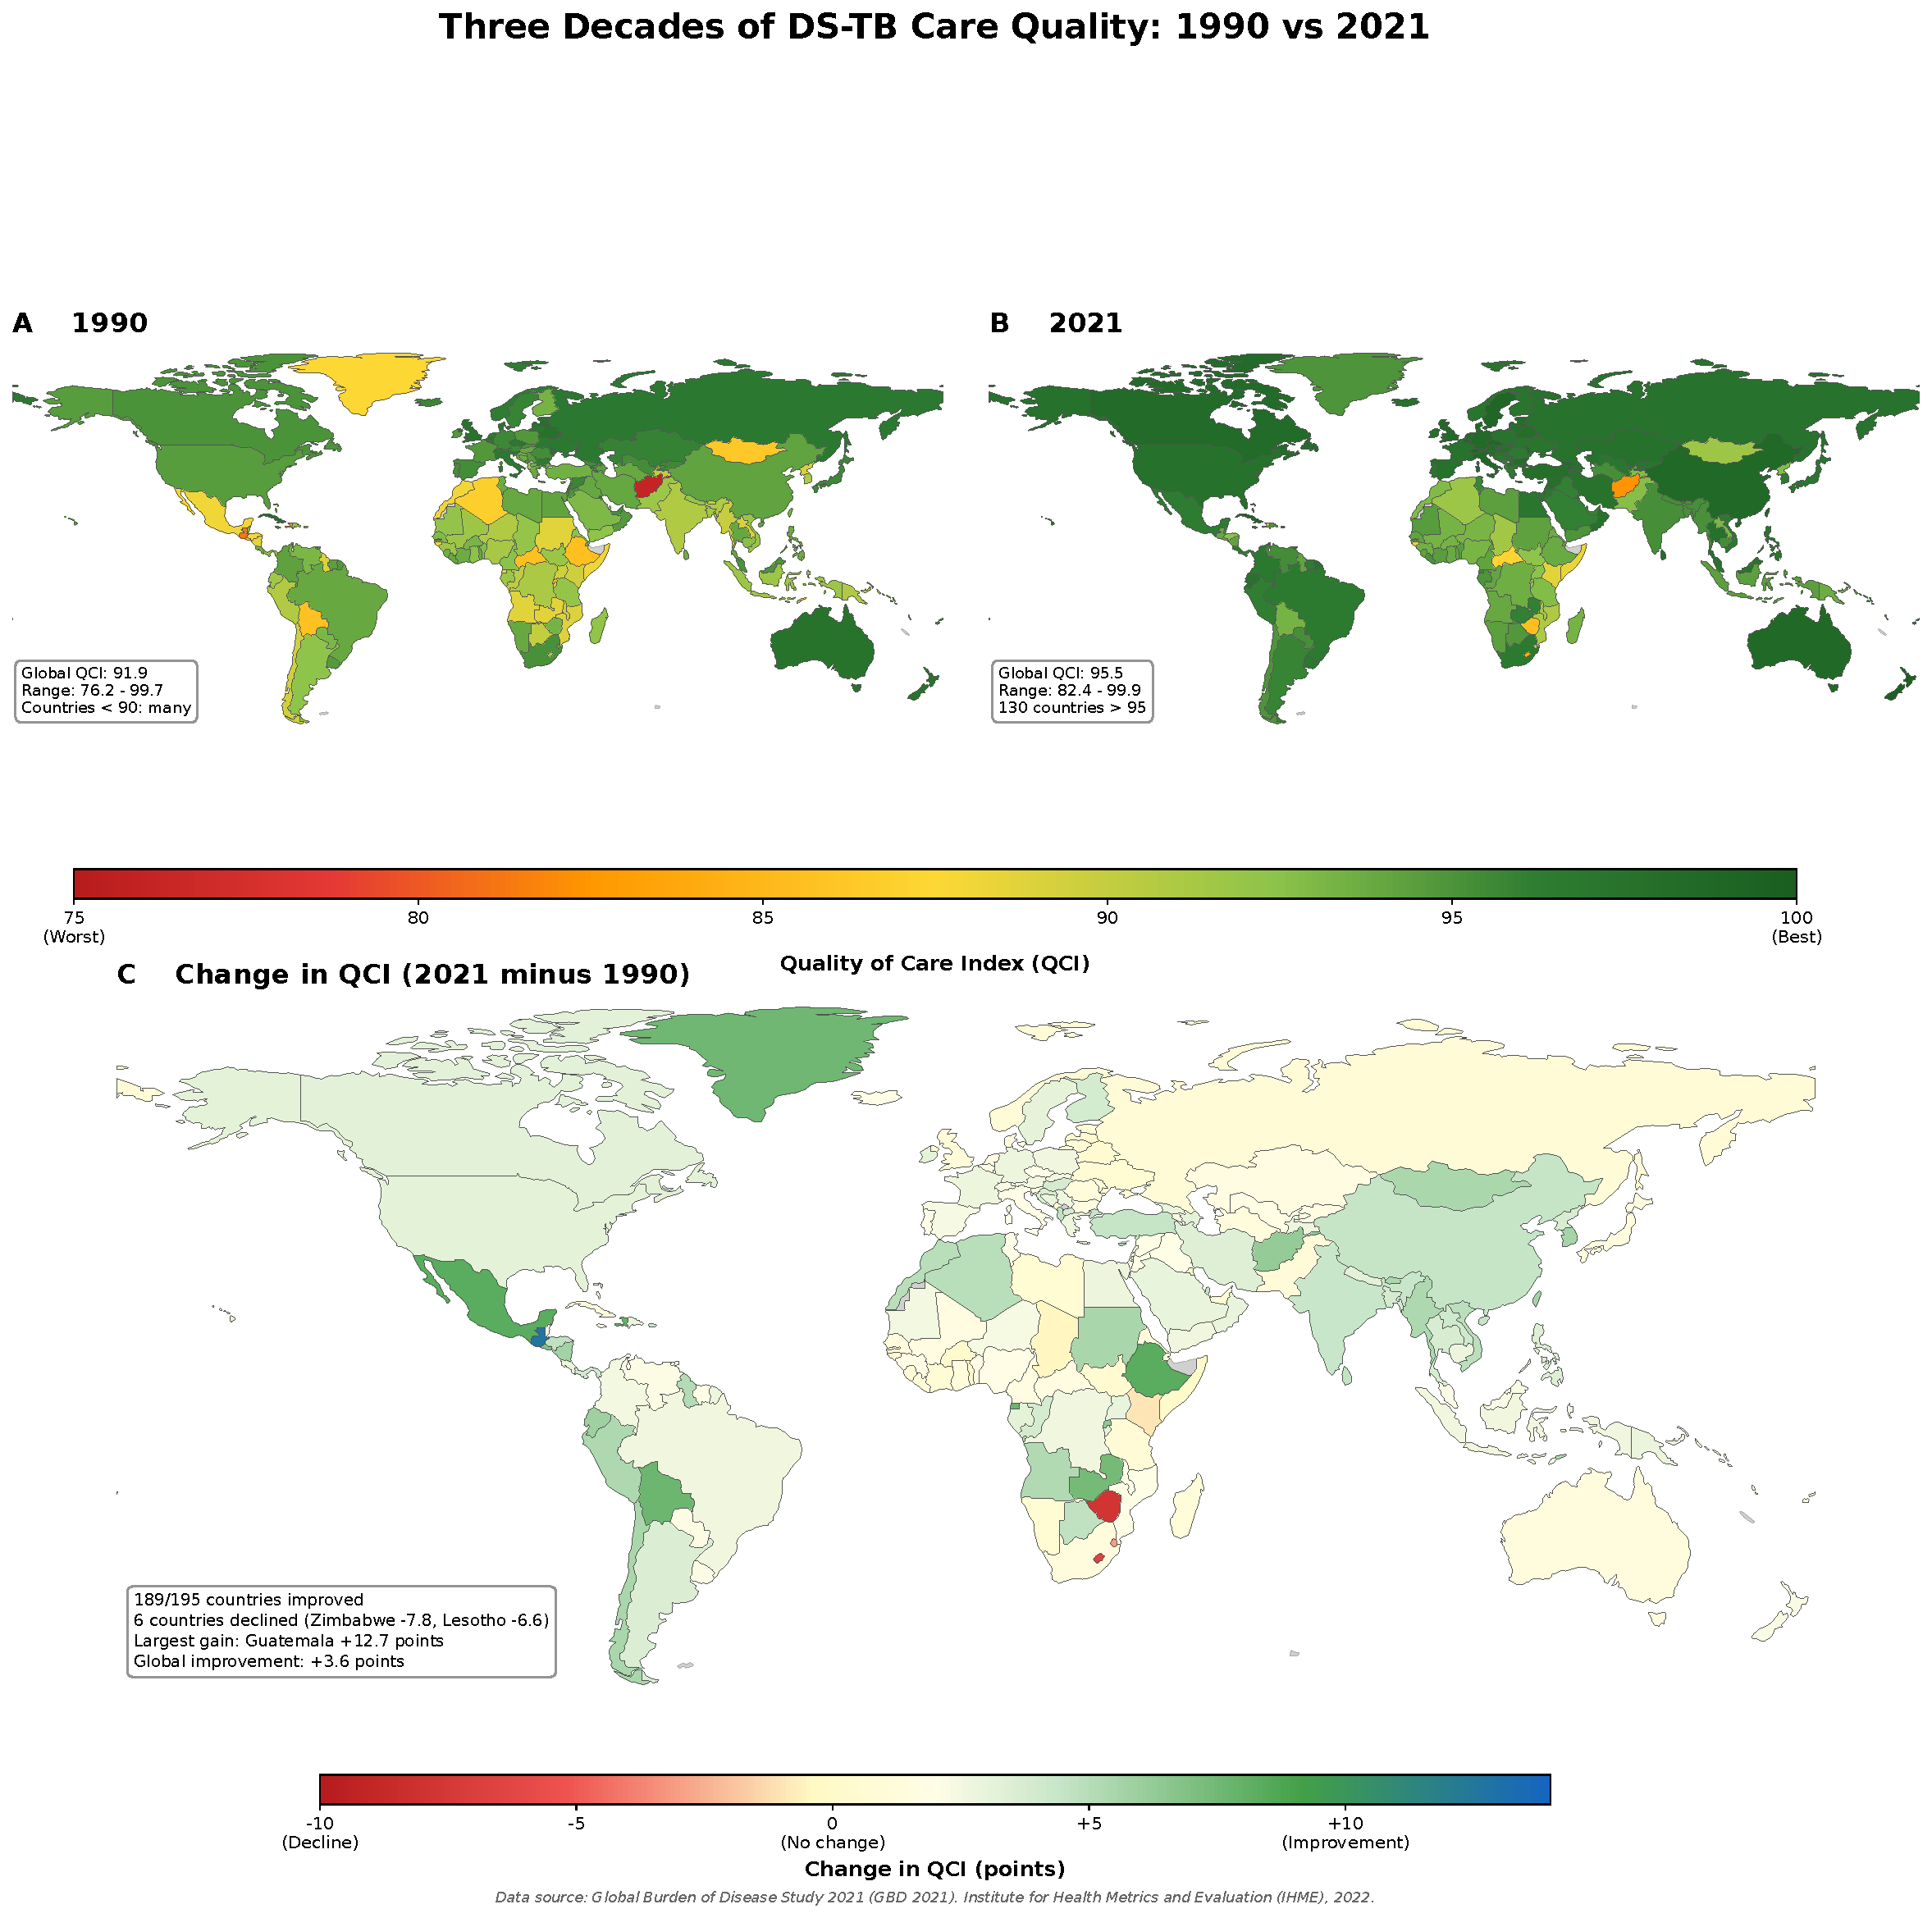
\includegraphics[width=\textwidth]{figure1_world_maps.pdf}
\caption{Three decades of DS-TB care quality: world maps comparing QCI in 1990 (Panel A) and 2021 (Panel B), with change map (Panel C). The shift from yellow/orange to deep green across most regions illustrates global improvement. Red in the change map identifies the six countries with declining QCI, notably Zimbabwe (--7.8 points) and Lesotho (--6.6 points).}
\label{fig:figure1}
\end{figure}

\clearpage

\begin{figure}[htbp]
\centering
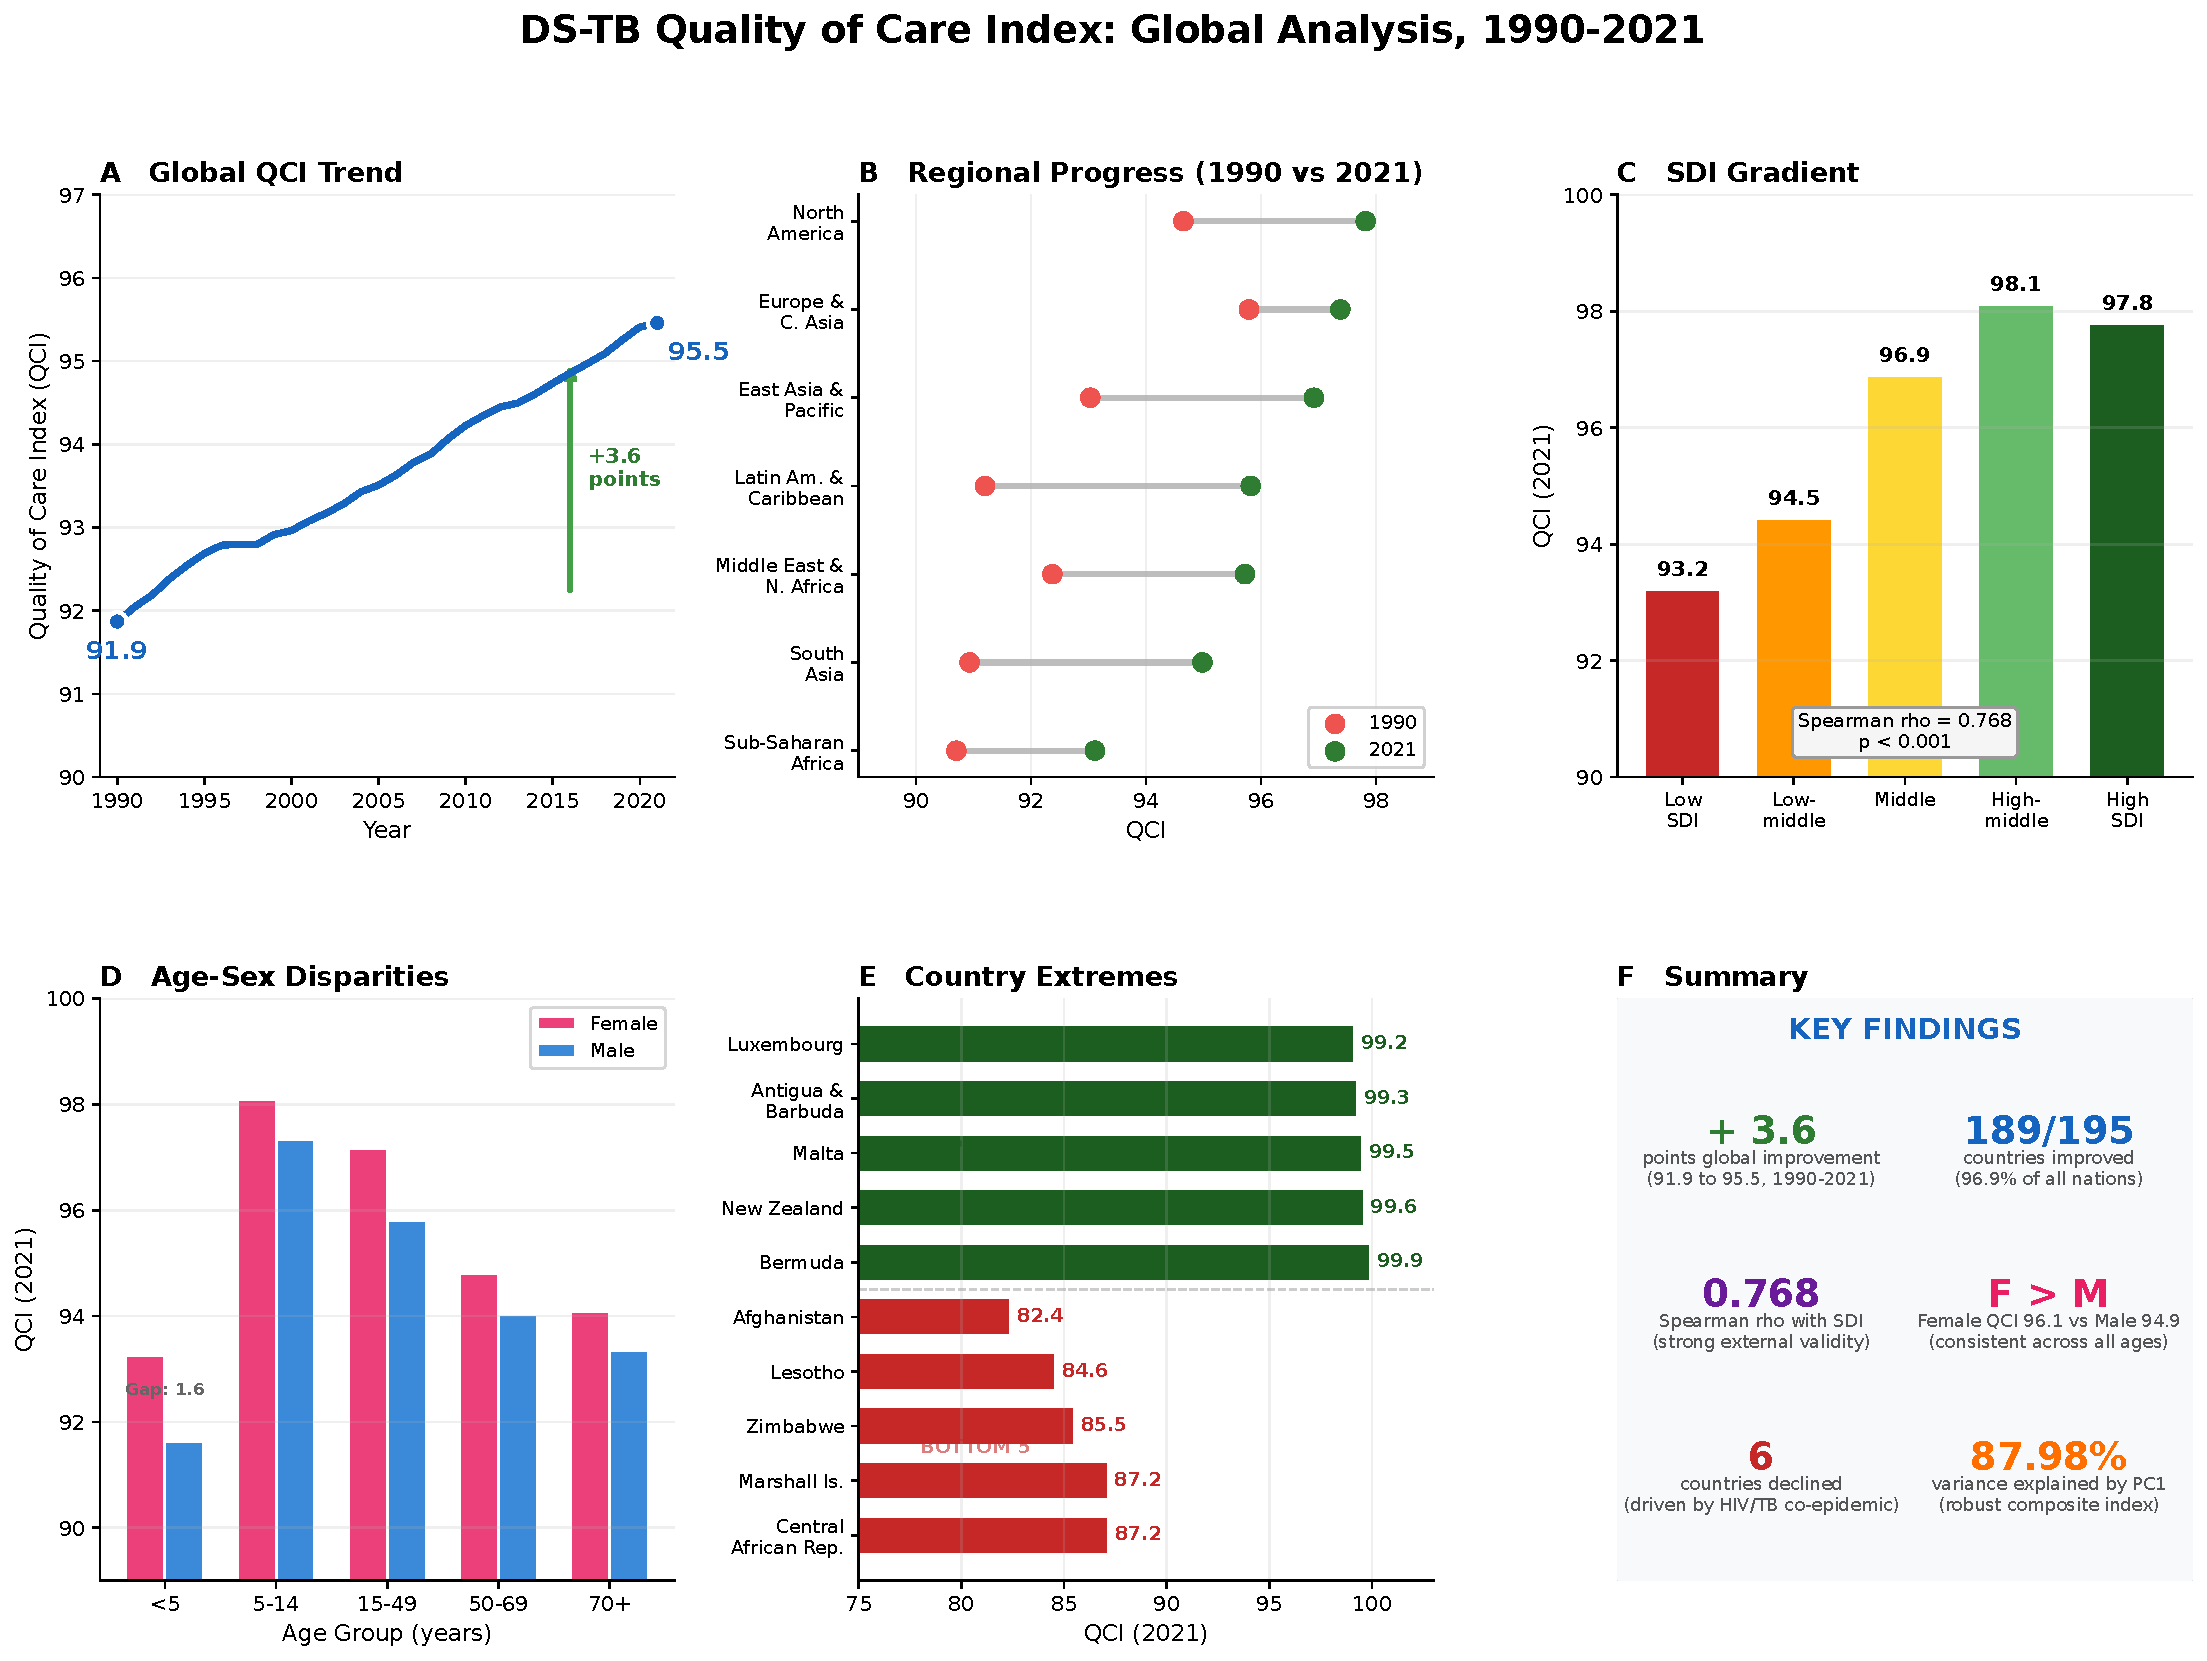
\includegraphics[width=\textwidth]{figure2_graphical_abstract.pdf}
\caption{Graphical abstract: six-panel summary of key findings. (A) Global QCI trend, (B) regional progress, (C) SDI gradient, (D) age-sex disparities, (E) country extremes, (F) summary statistics.}
\label{fig:figure2}
\end{figure}

\clearpage

\begin{figure}[htbp]
\centering
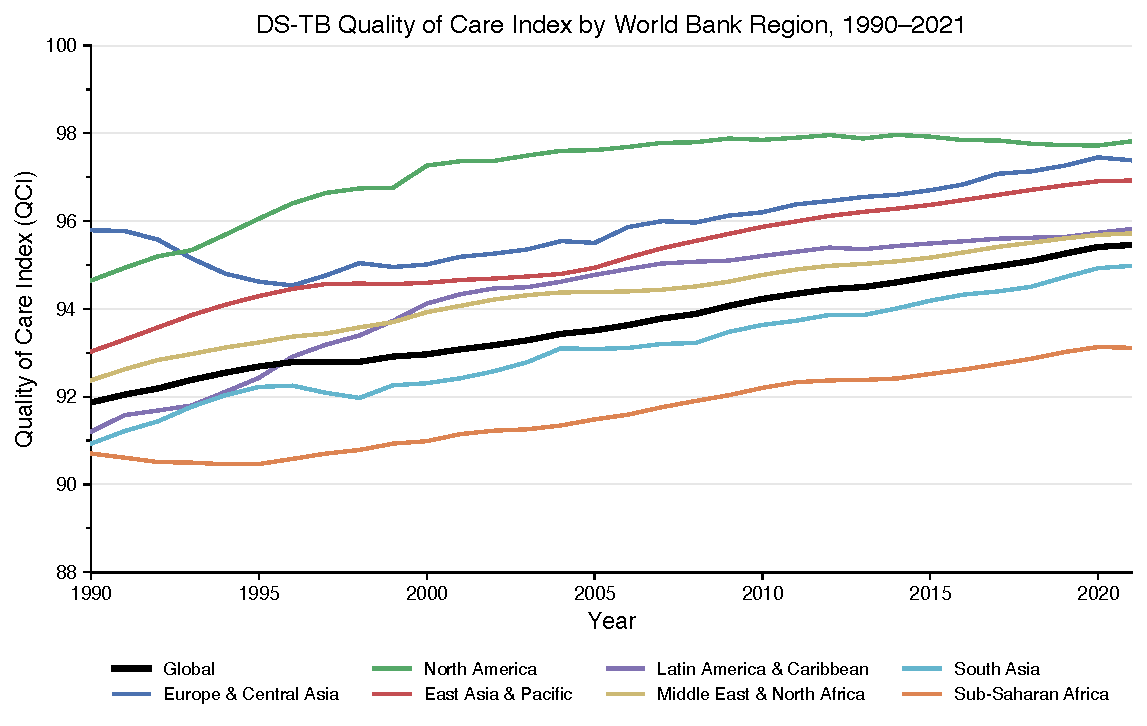
\includegraphics[width=\textwidth]{figure3_regional_qci_timeseries.pdf}
\caption{Age-standardised QCI for DS-TB by World Bank region, 1990--2021. Lines show QCI trends for each of seven World Bank regions, illustrating convergence over time with persistent gaps.}
\label{fig:figure3}
\end{figure}

\clearpage

\begin{figure}[htbp]
\centering
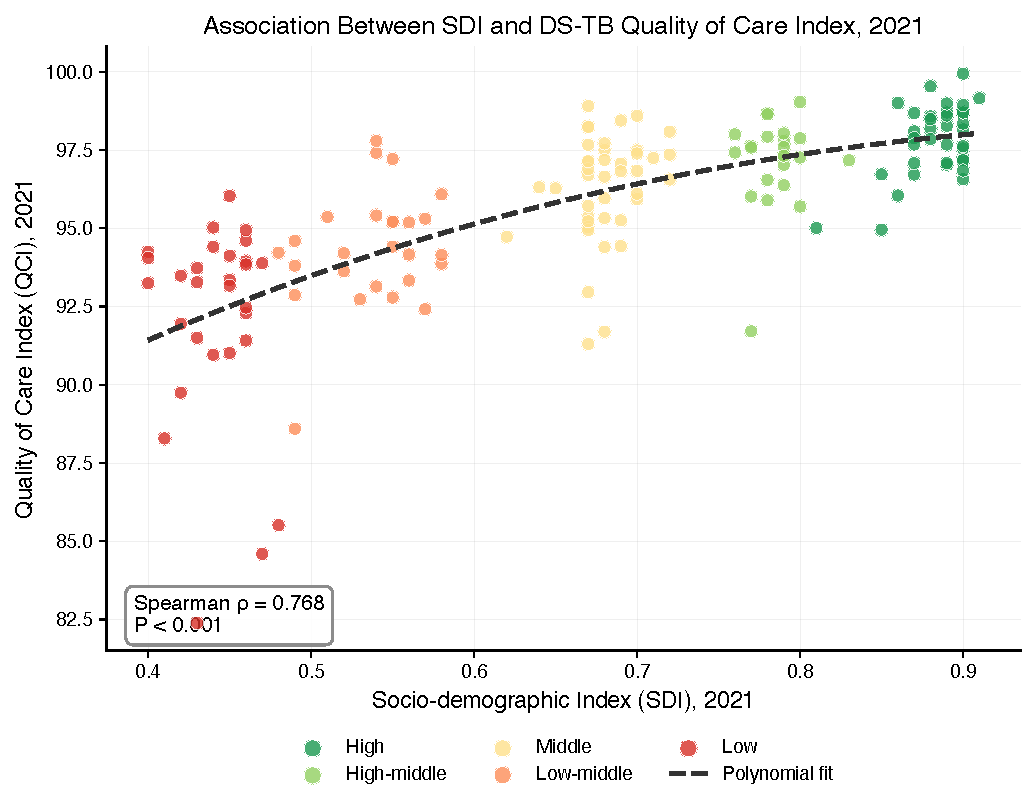
\includegraphics[width=\textwidth]{figure4_sdi_gradient_scatter.pdf}
\caption{Scatter plot of QCI (2021) versus SDI for 155 countries. Each point represents a country; colour indicates SDI group. Spearman rho = 0.768 (p = 2.03 $\times$ 10\textsuperscript{--31}).}
\label{fig:figure4}
\end{figure}

\clearpage

\begin{figure}[htbp]
\centering
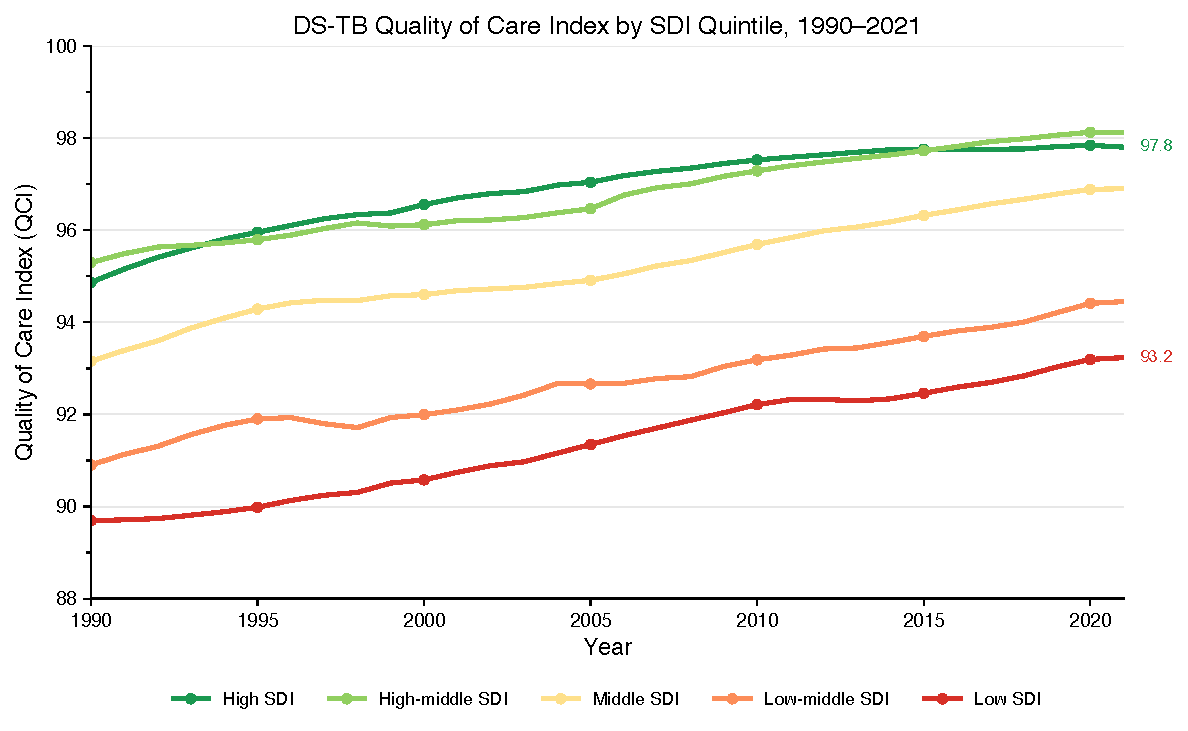
\includegraphics[width=\textwidth]{figure5_sdi_quintile_timeseries.pdf}
\caption{Age-standardised QCI by SDI quintile, 1990--2021. Time series showing convergence between low and high SDI groups, with faster improvement in low-SDI settings.}
\label{fig:figure5}
\end{figure}

\clearpage

\begin{figure}[htbp]
\centering
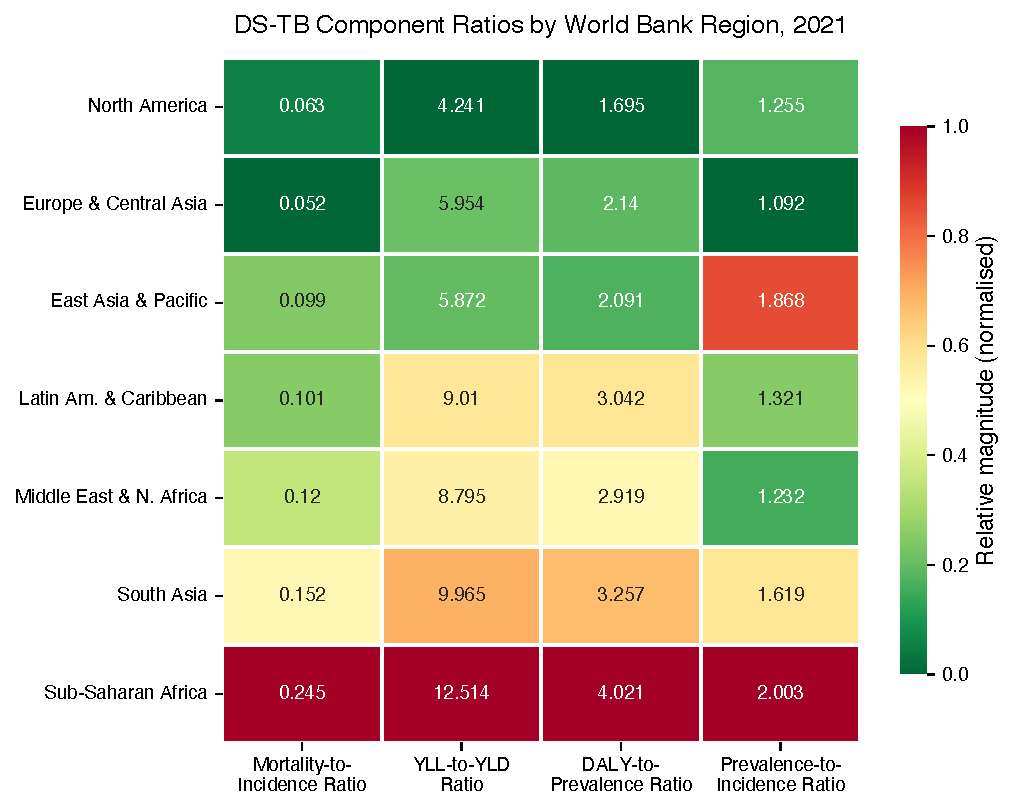
\includegraphics[width=\textwidth]{figure6_component_heatmap.pdf}
\caption{Component ratios (MIR, YLLtoYLD, DALtoPER) by World Bank region, 2021. Heatmap showing the gradient in each component, with Sub-Saharan Africa having the highest (worst) values across all three.}
\label{fig:figure6}
\end{figure}

\clearpage

\begin{figure}[htbp]
\centering
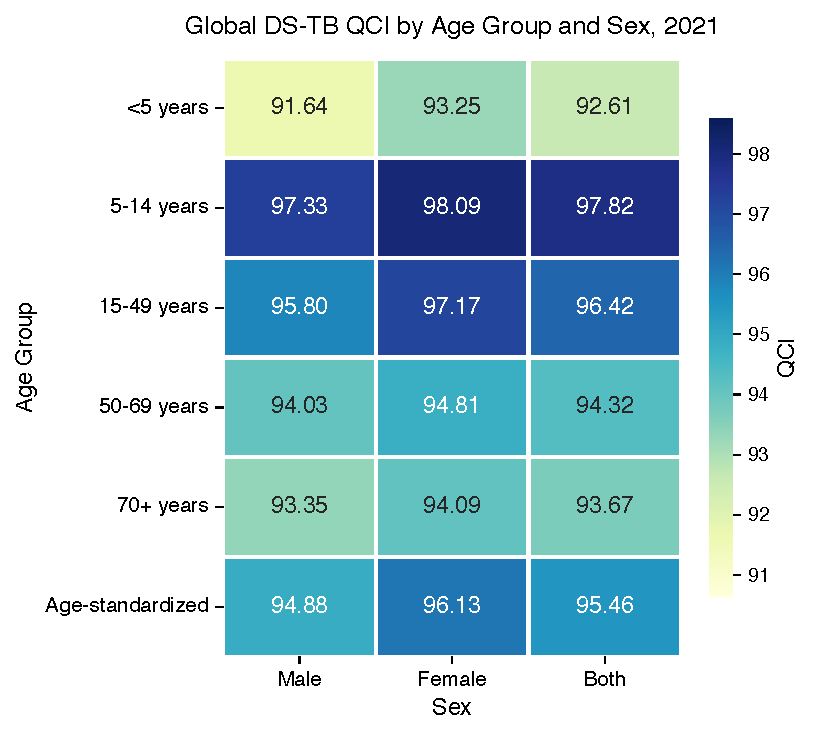
\includegraphics[width=\textwidth]{figure7_age_sex_heatmap.pdf}
\caption{QCI by age group and sex, global, 2021. Heatmap displaying the joint distribution of QCI across seven age groups and both sexes, highlighting the vulnerability of children under 5 years and older adults.}
\label{fig:figure7}
\end{figure}

\clearpage

\begin{figure}[htbp]
\centering
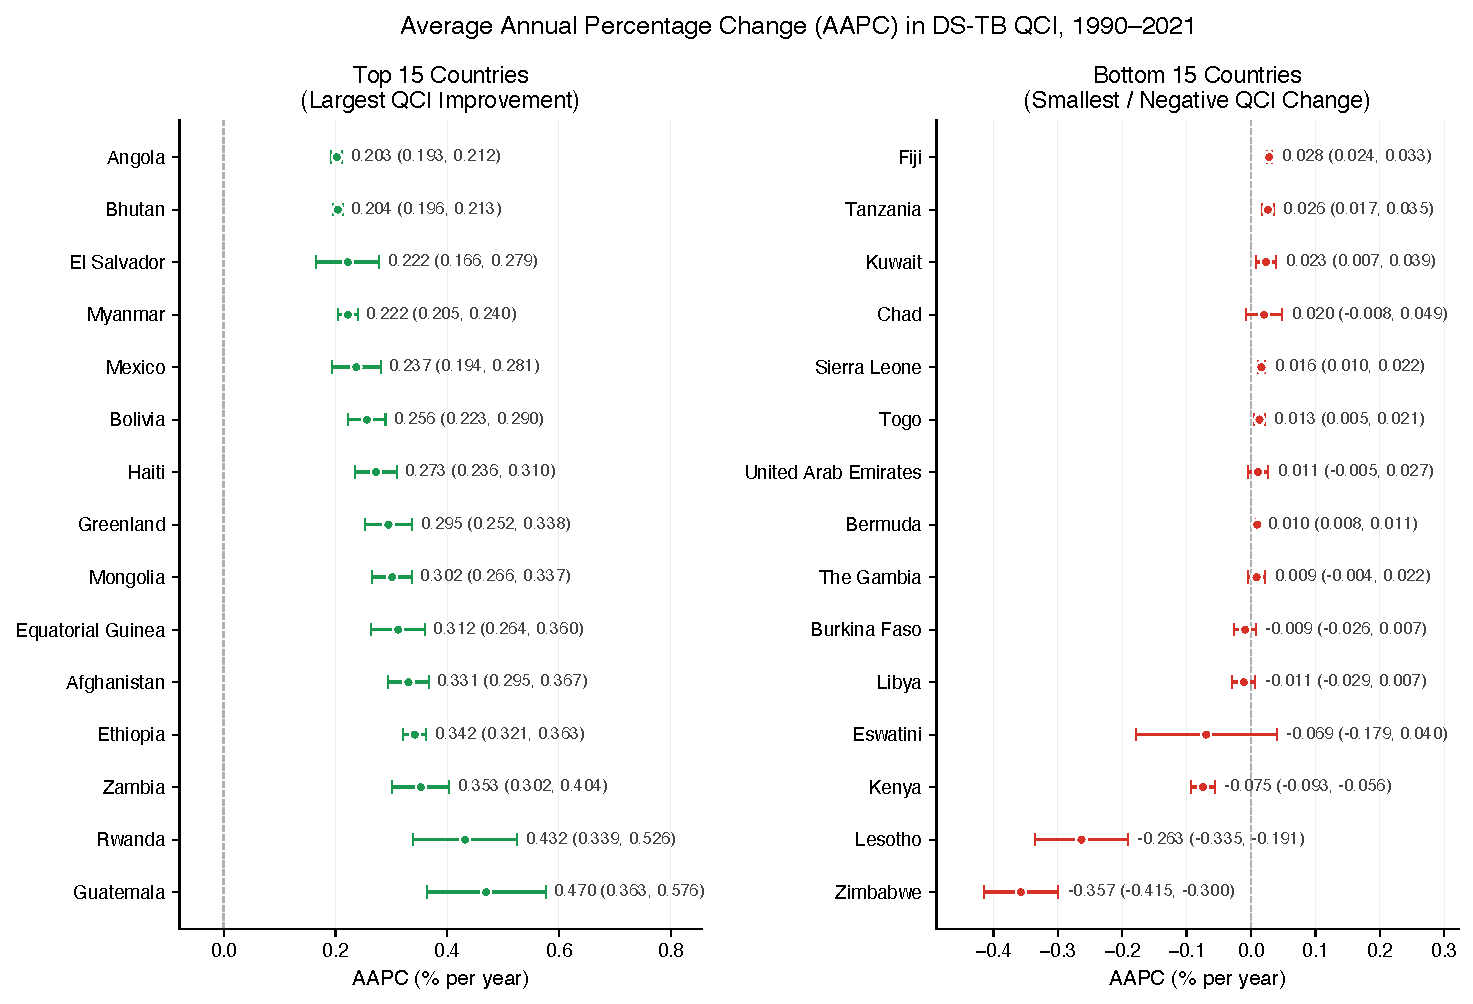
\includegraphics[width=\textwidth]{figure8_aapc_forest_plot.pdf}
\caption{Forest plot of country-level AAPC in QCI, 1990--2021. Countries sorted by AAPC with 95\% confidence intervals. Highlights the six countries with negative full-period AAPC.}
\label{fig:figure8}
\end{figure}

\clearpage

\begin{figure}[htbp]
\centering
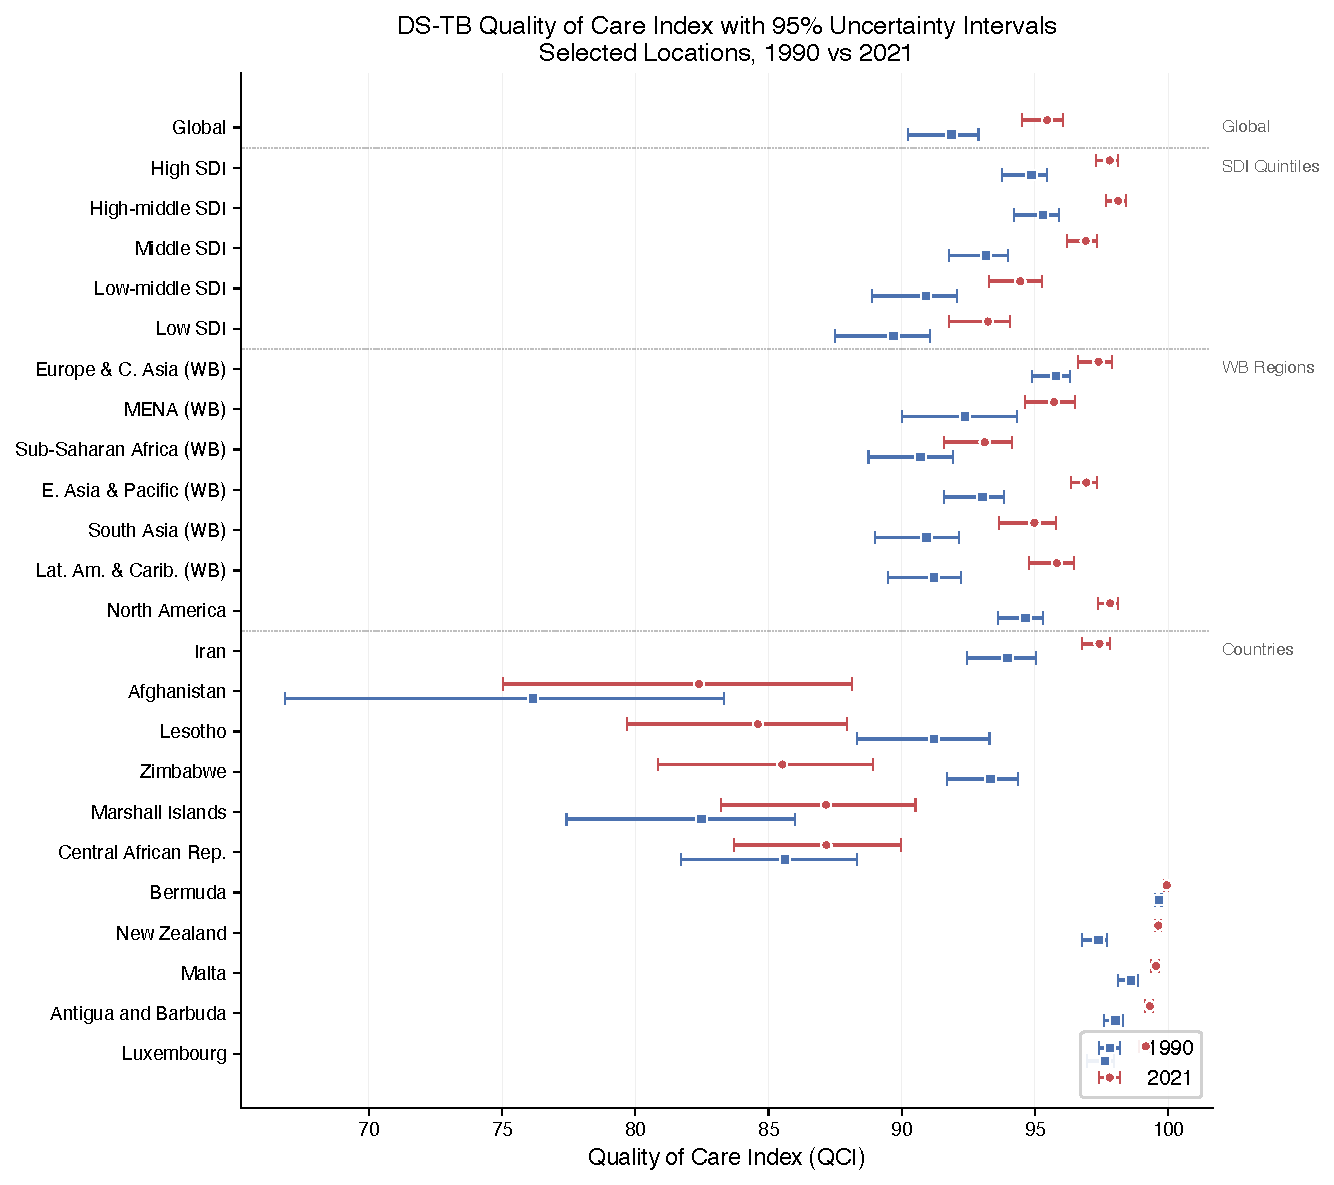
\includegraphics[width=\textwidth]{figure9_qci_uncertainty.pdf}
\caption{QCI uncertainty estimates for selected locations. Point estimates with 95\% uncertainty intervals from Monte Carlo simulation (1000 draws), showing wider intervals in data-sparse settings.}
\label{fig:figure9}
\end{figure}

%% ============================================================
%% REFERENCES
%% ============================================================

\clearpage

\begin{thebibliography}{34}

\bibitem{ref1}
World Health Organization. Global tuberculosis report 2023. Geneva: WHO; 2023.

\bibitem{ref2}
Pai M, Behr MA, Dowdy D, et al. Tuberculosis. \textit{Nat Rev Dis Primers} 2016; \textbf{2}: 16076.

\bibitem{ref3}
Kruk ME, Gage AD, Arsenault C, et al. High-quality health systems in the Sustainable Development Goals era: time for a revolution. \textit{Lancet Glob Health} 2018; \textbf{6}: e1196--252.

\bibitem{ref4}
World Health Organization. The End TB Strategy. Geneva: WHO; 2015.

\bibitem{ref5}
Subbaraman R, Nathavitharana RR, Mayer KH, et al. Constructing care cascades for active tuberculosis: a strategy for program monitoring and identifying gaps in quality of care. \textit{PLoS Med} 2019; \textbf{16}: e1002754.

\bibitem{ref6}
GBD 2019 Healthcare Access and Quality Collaborators. Assessing performance of the Healthcare Access and Quality Index, overall and by select age groups, for 204 countries and territories, 1990--2019: a systematic analysis from the Global Burden of Disease Study 2019. \textit{Lancet Glob Health} 2022; \textbf{10}: e1715--43.

\bibitem{ref7}
Global Burden of Disease Collaborative Network. Global Burden of Disease Study 2021 (GBD 2021) Results. Seattle, United States: Institute for Health Metrics and Evaluation (IHME), 2022. Available from \url{https://vizhub.healthdata.org/gbd-results/}.

\bibitem{ref8}
GBD 2021 Diseases and Injuries Collaborators. Global, regional, and national incidence, prevalence, and years lived with disability for 354 diseases and injuries for 195 countries and territories, 1990--2021: a systematic analysis for the Global Burden of Disease Study 2021. \textit{Lancet} 2024; \textbf{403}: 2162--203.

\bibitem{ref9}
GBD 2021 Causes of Death Collaborators. Global, regional, and national age-sex-specific mortality for 288 causes of death, 1990--2021: a systematic analysis for the Global Burden of Disease Study 2021. \textit{Lancet} 2024; \textbf{403}: 2100--32.

\bibitem{ref10}
Lawn SD, Zumla AI. Tuberculosis. \textit{Lancet} 2011; \textbf{378}: 57--72.

\bibitem{ref11}
Kwan CK, Ernst JD. HIV and tuberculosis: a deadly human syndemic. \textit{Clin Microbiol Rev} 2011; \textbf{24}: 351--76.

\bibitem{ref12}
Raviglione M, Sulis G. Tuberculosis 2015: burden, challenges and strategy for control and elimination. \textit{Infect Dis Rep} 2016; \textbf{8}: 6570.

\bibitem{ref13}
Talwar A, Tsang CA, Price SF, et al. Tuberculosis -- United States, 2018. \textit{MMWR Morb Mortal Wkly Rep} 2019; \textbf{68}: 257--62.

\bibitem{ref14}
Corbett EL, Watt CJ, Walker N, et al. The growing burden of tuberculosis: global trends and interactions with the HIV epidemic. \textit{Arch Intern Med} 2003; \textbf{163}: 1009--21.

\bibitem{ref15}
Horton KC, MacPherson P, Houben RMGJ, et al. Sex differences in tuberculosis burden and notifications in low- and middle-income countries: a systematic review and meta-analysis. \textit{PLoS Med} 2016; \textbf{13}: e1002119.

\bibitem{ref16}
Nhamoyebonde S, Leslie A. Biological differences between the sexes and susceptibility to tuberculosis. \textit{J Infect Dis} 2014; \textbf{209} (suppl 3): S100--6.

\bibitem{ref17}
Dodd PJ, Yuen CM, Sismanidis C, et al. The global burden of tuberculosis mortality in children: a mathematical modelling study. \textit{Lancet Glob Health} 2017; \textbf{5}: e898--906.

\bibitem{ref18}
Marais BJ, Gie RP, Schaaf HS, et al. The natural history of childhood intra-thoracic tuberculosis: a critical review of literature from the pre-chemotherapy era. \textit{Int J Tuberc Lung Dis} 2004; \textbf{8}: 392--402.

\bibitem{ref19}
World Health Organization. Global tuberculosis report 2021. Geneva: WHO; 2021.

\bibitem{ref20}
McQuaid CF, McCreesh N, Read JM, et al. The potential impact of COVID-19-related disruption on tuberculosis burden. \textit{Eur Respir J} 2020; \textbf{56}: 2001718.

\bibitem{ref21}
Jolliffe IT, Cadima J. Principal component analysis: a review and recent developments. \textit{Philos Trans A Math Phys Eng Sci} 2016; \textbf{374}: 20150202.

\bibitem{ref22}
Fullman N, Yearwood J, Abay SM, et al. Measuring performance on the Healthcare Access and Quality Index for 195 countries and territories and selected subnational locations: a systematic analysis from the Global Burden of Disease Study 2016. \textit{Lancet} 2018; \textbf{391}: 2236--71.

\bibitem{ref23}
Hogan AB, Jewell BL, Sherrard-Smith E, et al. Potential impact of the COVID-19 pandemic on HIV, tuberculosis, and malaria in low-income and middle-income countries: a modelling study. \textit{Lancet Glob Health} 2020; \textbf{8}: e1132--41.

\bibitem{ref24}
Glaziou P, Floyd K, Raviglione MC. Global epidemiology of tuberculosis. \textit{Semin Respir Crit Care Med} 2018; \textbf{39}: 271--85.

\bibitem{ref25}
Uplekar M, Weil D, Lonnroth K, et al. WHO's new End TB Strategy. \textit{Lancet} 2015; \textbf{385}: 1799--801.

\bibitem{ref26}
Neyrolles O, Quintana-Murci L. Sexual inequality in tuberculosis. \textit{PLoS Med} 2009; \textbf{6}: e1000199.

\bibitem{ref27}
Rajagopalan S. Tuberculosis and aging: a global health problem. \textit{Clin Infect Dis} 2001; \textbf{33}: 1034--39.

\bibitem{ref28}
Donabedian A. The quality of medical care: how can it be assessed? \textit{JAMA} 1988; \textbf{260}: 1743--48.

\bibitem{ref29}
Marrero A, Caminero JA, Rodr{\'\i}guez R, Billo NE. Towards elimination of tuberculosis in a low-income country: the experience of Cuba, 1962--97. \textit{Thorax} 2000; \textbf{55}: 39--45.

\bibitem{ref30}
Datiko DG, Lindtj{\o}rn B. Health extension workers improve tuberculosis case detection and treatment success in southern Ethiopia: a community randomized trial. \textit{PLoS One} 2009; \textbf{4}: e5443.

\bibitem{ref31}
L{\"o}nnroth K, Migliori GB, Abubakar I, et al. Towards tuberculosis elimination: an action framework for low-incidence countries. \textit{Eur Respir J} 2015; \textbf{45}: 928--52.

\bibitem{ref32}
GBD 2015 SDI Collaborators. Measuring the health-related Sustainable Development Goals in 188 countries: a baseline analysis from the Global Burden of Disease Study 2015. \textit{Lancet} 2016; \textbf{388}: 1813--50.

\bibitem{ref33}
Zar HJ, Hanslo D, Apolles P, Swingler G, Hussey G. Induced sputum versus gastric lavage for microbiological confirmation of pulmonary tuberculosis in infants and young children: a prospective study. \textit{Lancet} 2005; \textbf{365}: 130--34.

\bibitem{ref34}
World Health Organization. Guidance for national tuberculosis programmes on the management of tuberculosis in children, 2nd edn. Geneva: WHO; 2014.

\end{thebibliography}

%% ============================================================
%% END MATTER
%% ============================================================

\clearpage

\section*{Declaration of interests}

We declare no competing interests.

\section*{Data sharing}

All input data used in this study are publicly available through the GBD Results Tool (\url{https://vizhub.healthdata.org/gbd-results/}).\textsuperscript{7} The analytical code used to construct the QCI, including PCA transformation, Monte Carlo uncertainty propagation, and all visualisations, will be made available in a public repository upon publication. [Add repository URL, e.g., GitHub or Zenodo DOI.]

\section*{Contributors}

[To be completed using CRediT taxonomy -- e.g., Conceptualisation, Data curation, Formal analysis, Methodology, Visualisation, Writing (original draft), Writing (review and editing), Supervision. All authors should review and approve the final manuscript.]

\section*{GATHER compliance}

This study was conducted in accordance with the Guidelines for Accurate and Transparent Health Estimates Reporting (GATHER). A completed GATHER checklist is provided in the Supplementary Materials.

\section*{Ethical approval}

Ethical approval was not required for this study as it exclusively used publicly available, de-identified, aggregate data from the GBD 2021 Study.

\end{document}
